\documentclass{classrep}
\usepackage[utf8x]{inputenc}
\usepackage[a4paper, left=1.5cm, right=1.5cm, top=1.0cm, bottom=1.5cm, headsep=0.5cm, headheight=13pt]{geometry}
\usepackage{amsmath, amsthm, amssymb, amsfonts}
\usepackage{graphicx}
\usepackage{float}
\usepackage{listings}
\usepackage{caption}
\usepackage{lipsum} % for dummy text only


\lstdefinelanguage{VHDL}{
	morekeywords={
		library,use,all,entity,is,port,in,out,end,architecture,of,if,downto,process,when,then,elsif,else,
		begin,and,LIBRARY,USE,ALL,ENTITY,IS,PORT,IN,OUT,END,ARCHITECTURE,OF,BEGIN,AND
	},
	morecomment=[l]--
}

\usepackage{xcolor}
\colorlet{keyword}{blue!100!black!80}
\colorlet{comment}{green!90!black!90}
\lstdefinestyle{vhdl}{
	language     = VHDL,
	basicstyle   = \ttfamily,
	keywordstyle = \color{keyword}\bfseries,
	 stringstyle=\ttfamily\color{red!50!brown},
	commentstyle = \color{comment}
}
\lstset{language=VHDL,style=vhdl,literate=%
	*{0}{{{\color{red!20!violet}0}}}1
	{1}{{{\color{red!20!violet}1}}}1
	{2}{{{\color{red!20!violet}2}}}1
	{3}{{{\color{red!20!violet}3}}}1
	{4}{{{\color{red!20!violet}4}}}1
	{5}{{{\color{red!20!violet}5}}}1
	{6}{{{\color{red!20!violet}6}}}1
	{7}{{{\color{red!20!violet}7}}}1
	{8}{{{\color{red!20!violet}8}}}1
	{9}{{{\color{red!20!violet}9}}}1}
\lstset{basicstyle=\ttfamily\footnotesize,breaklines=true}
\lstset{framextopmargin=4pt,frame=top,frame=bottom,captionpos=t}
\DeclareCaptionFormat{listing}{\rule{\dimexpr\textwidth\relax}{0.4pt}\par\vskip1pt#1#2#3}
\captionsetup[lstlisting]{format=listing,singlelinecheck=false, margin=0pt, font={sf},labelsep=space,labelfont=bf}


\usepackage{hyperref} % musi być na końcu
\hypersetup{pdfborder={0 0 0 0}}
%%%%%%%%%%%%%
%%%%%%%%%%%%
%%%%%%%%


\studycycle{Elektronika i Telekomunikacja, studia dzienne, mgr II st.}
\coursesemester{I}

\coursename{Programowalne układy cyfrowe}
\courseyear{2014/2015}

\courseteacher{mgr. Tomaszewski Grzegorz}
\coursegroup{poniedziałek, 14:00}

\author{
  \studentinfo{Witold Olechowski}{127517} \and
  \studentinfo{Tomasz Marecik}{127374}
}

\title{Zadanie : Do setki !!!!!!!!!!!!}

%\lstinputlisting{block1.vhdl}
%\vskip 2\baselineskip

\begin{document}
\maketitle

\section{Cel ćwiczenia:}
% tu tekst
\lipsum[1]

\section{Pierwszy wariant realizacji zadania}
\label{sec:pierw} % tworzy etykiete do ktorej sie mozna odwolac 

\begin{figure}[H]  % H - obraz dokladnie w tym miejscu, t - u gory etc..
	\centering
	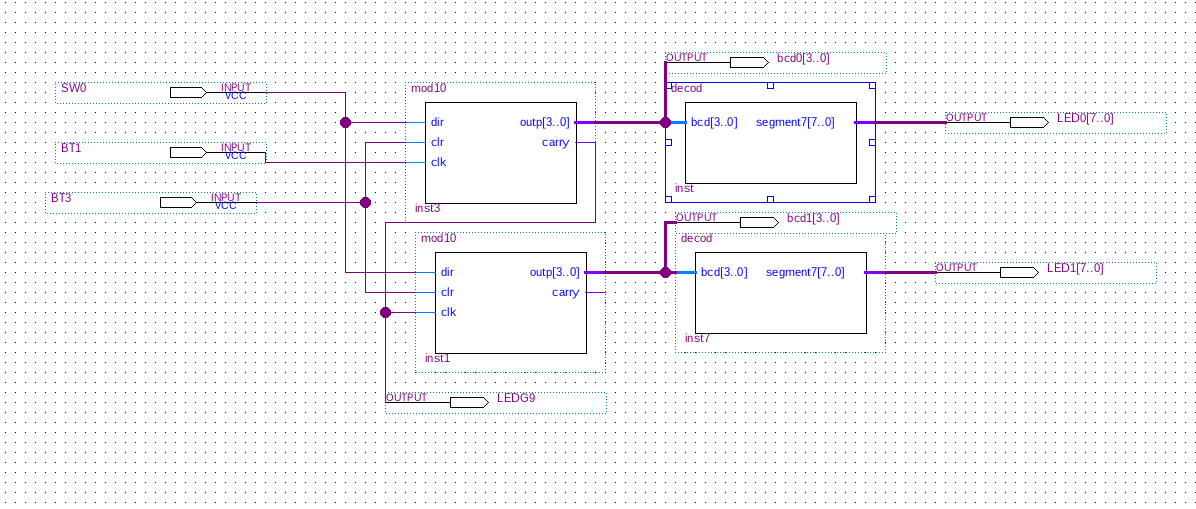
\includegraphics[width=1.0\linewidth]{blok}  % zalacza grafike z rozciagnieciem na cala linie  
	\caption{Schemat blokowy układu }
	\label{fig:block_bcd_segment}
\end{figure}

\lipsum[2]

\lstinputlisting[label=lst_mod10,caption=Licznik modulo 10 ,language=VHDL]{mod10.vhd}

\lipsum[3]

\lstinputlisting[label=lst_mod10,caption=Dekoder bcd to 7 segment ,language=VHDL]{decod.vhd}


\subsection{Przebiegi czasowe układu:}
\lipsum[5]
\begin{figure}[H]
	\centering
	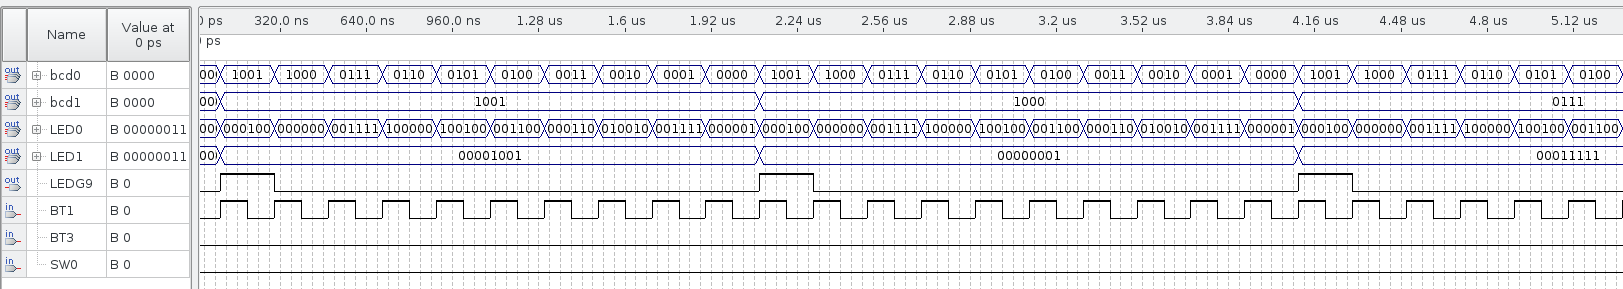
\includegraphics[width=1.0\linewidth]{up_down_1}
	\caption{liczy do tylu}
	\label{fig:symhex0}
\end{figure}

\lipsum[6]

\begin{figure}[H]
	\centering
	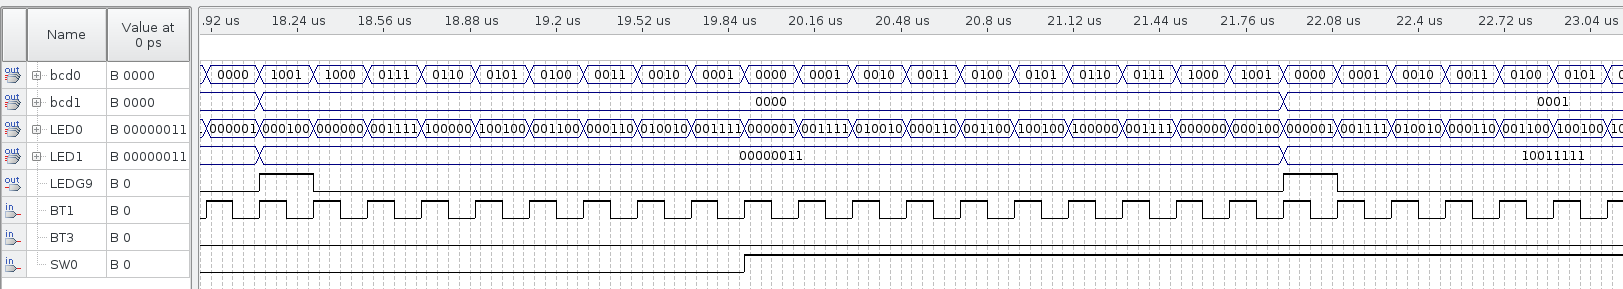
\includegraphics[width=1.0\linewidth]{up_down_2}
	\caption{liczy do tylu do 0 i do przodu patrz na bt3}
	\label{fig:symhex0}
\end{figure}

\lipsum[7]

\begin{figure}[H]
	\centering
	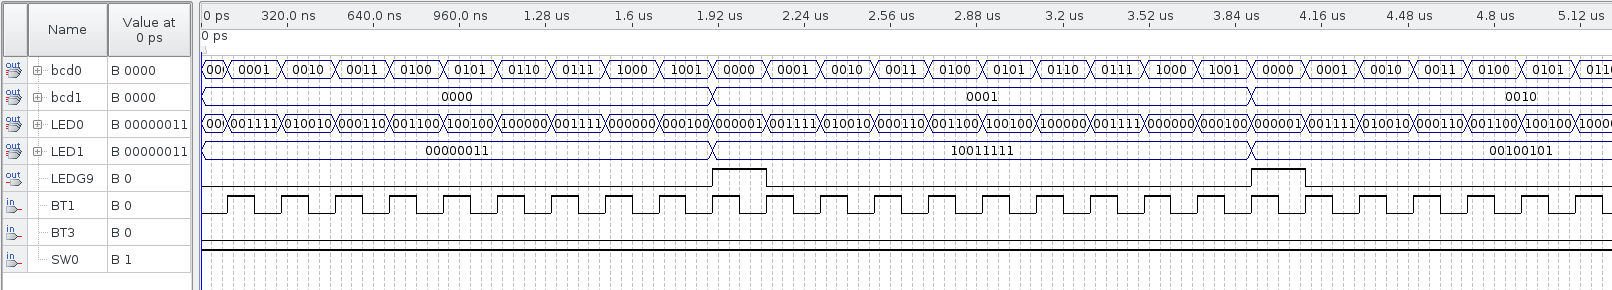
\includegraphics[width=1.0\linewidth]{up_down_inv_1}
	\caption{liczy do przodu }
	\label{fig:symhex0}
\end{figure}

\lipsum[7]

\begin{figure}[H]
	\centering
	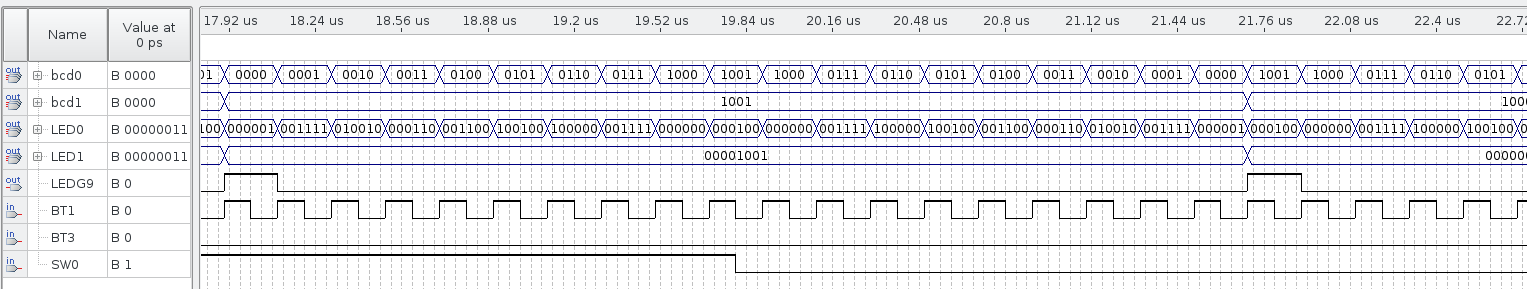
\includegraphics[width=1.0\linewidth]{up_down_inv_2}
	\caption{liczy do przodu  oo\_O i do tylu}
	\label{fig:symhex0}
\end{figure}

\section{Wnioski}

\lipsum[8]

\begin{thebibliography}{0}
  \bibitem{l2short} John Wiley and Sons Publishers.
    \textsl{Digital Design,} University of California, Riverside, 2007
\end{thebibliography}
\end{document}
